\chapter{Anti-aliasing}
	L'anti-aliasing est un problème pour tout framework d'édition d'image; la pluspart
	des problèmes et des solutions sont donc connues. 
	Cependant l'édition d'image gigapixel est un problème relativement nouveau qui
	apporte des nouveaux problèmes qui méritent notre attention. C'est sur ces problèmes
	que nous nous sommes concentrés dans ce chapitre. 

	La première chose à remarquer c'est que contrairement au raytracing dont il s'inspire,
	l'algorithme de rasterisation de ce framework n'a aucun mécanisme
	particulier pour gérer l'antialiasing. Il revient donc aux opérations de s'assurer que
	leur résultat est correctement anti-aliasé. La première partie examinera les 
	problèmes que l'on peut résoudre au niveau des opérations. Nous examinerons ensuite 
	une modification de l'algorithme de rasterisation pour apporter une solution globale à
	l'antialiasing.

	\section{Anti-aliasing des opérations}

	La seule opération que nous aillons testé étant le dessin de disque avec 
	dégradé, on retrouvera dans cette section les problèmes posés par cette opération.
	Cependant nombre de ces problèmes sont d'ordre géneral, et leurs solutions peuvent
	s'appliquer à d'autres opérations de dessin de primitives. 

		\begin{figure}[ht]
			\centering
			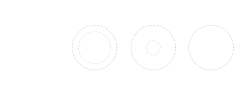
\includegraphics[width=\textwidth]{images/brushes} 
			\caption{La primitive de dessin}
			\label{fig:brush}
		\end{figure}
	La primitive de dessin utilisée est représentée à la figure~\ref{fig:brush}, page~\pageref{fig:brush}.
	
	Les paramètres qui la définissent sont sa position, sa couleur, son opacité globale, 
	son rayon interne qui définit une zone de couleur unie, et son rayon externe. Entre le rayon interne
	et externe, se trouve un dégradé d'opacité de profil gaussien.

	\subsection{Problèmes de bandes}
		S'il n'est pas fait correctement, le dessin de dégradés fait apparaître des
		bandes à l'écran. La cause est la quantisation 8bit du dégradé. Celle-ci se
		fait à deux endroits: Lors de la rasterisation, et lors de l'affichage. Ce qui veut
		dire qu'utiliser un format 32bit pour la rasterisation n'est pas suffisant pour
		éviter l'apparition de bandes lors de l'affichage à l'écran. 

		\begin{figure}[ht]
			\centering
			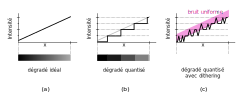
\includegraphics[width=\textwidth]{images/degrades} 
			\caption{Dégradés et dithering}
			\label{fig:dithering}
		\end{figure}

		Ce problème est illustré à la figure~\ref{fig:dithering}, page~\pageref{fig:dithering}.
		Le schéma (a) montre un dégradé linéaire idéal. Le schéma (b) montre l'effet 
		d'une quantisation sur ce dégradé. 

		Il s'agit là d'un problème largement connu et la solution l'est tout autant,
		et s'appelle le \emph{dithering}. Il s'agit d'ajouter à l'intensité de chaque pixel
		un bruit d'amplitude égale au niveau de quantisation, et ce avant l'étape
		de quantisation. Cette technique est illustrée sur le schéma (c) de la figure~\ref{fig:dithering} 

		Le bruit ajouté étant de très faible amplitude, il est imperceptible. mais il permet de diffuser
		les frontières entre les niveaux de quantisation.

		Le bruit utilisé pour l'implémentation est la fonction \emph{rand()} de la norme
		\emph{POSIX} qui a l'inconvénient de ne pas être très rapide à calculer. Une amélioration possible est de
		choisir un \emph{motif aléatoire}  de la taille d'un tile dans un ensemble de motifs
		précalculés. Il faut faire attention lors de la génération de ces motifs, car il faut éviter
		que leur supperposition lors de l'utilisation de plusieurs opérations en série
		ne fasse pas apparaitre de motifs visibles. pour cela il faut que la somme des pixels de sur l'ensemble
		des motifs soit égale à une valeur constante pour tous les pixels. 

	\subsection{Problèmes d'échelle}
		Le problème dans le rendu d'images gigapixel est qu'une primitive doit pouvoir être
		rendue à toute sorte d'échelles, de plusieurs milliers de pixels de large à beaucoup
		moins qu'un pixel. 

		Si le dessin de primitives de très grande taille ne pose pas de problèmes, les très
		petites en posent de nombreux lorsque leur taille approche du pixel.

		\subsubsection{Couverture du pixel}
			\begin{figure}[ht]
				\centering
				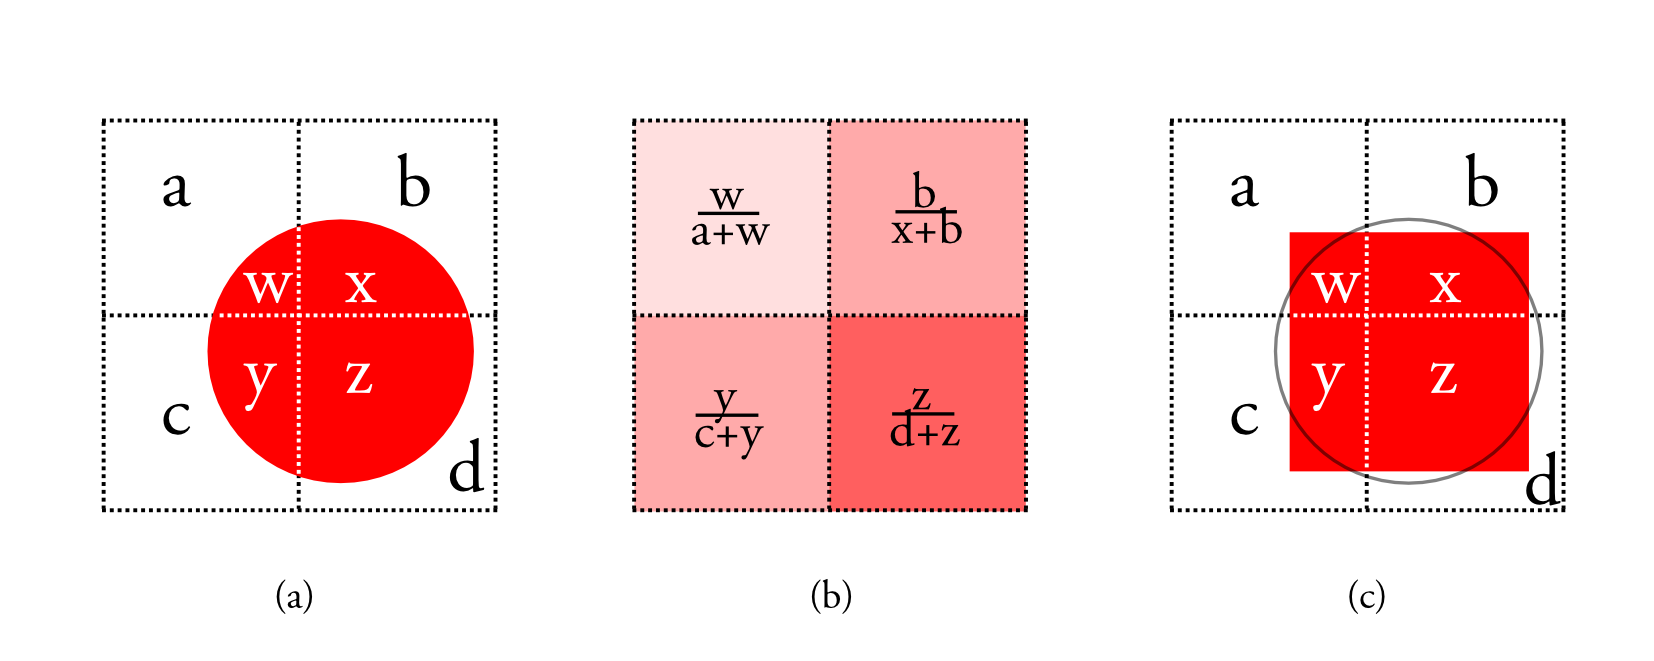
\includegraphics[width=\textwidth]{images/couverture-pixels} 
				\caption{Antialiasing de très petites primitives}
				\label{fig:couverture}
			\end{figure}
			Lorsque la primitive a une taille proche d'un pixel, elle peut couvrir partiellement
			plusieurs pixels. Ceci est illustré sur le schéma (a), de la figure~\ref{fig:couverture},
			page~\pageref{fig:couverture}

			La meilleure solution pour rasteriser une telle figure est de colorer les pixels partiellement
			couverts de manière proportionelle au rapport de l'aire de la primitive et du pixel, comme 
			illustré sur le schémà (b) de la figure~\ref{fig:couverture}.
			
			La solution exacte nécessite de calculer l'aire de l'intersection d'un disque et d'un carré. 
			La formule qui permet de calculer cela de manière analytique est malheureusement trop complexe pour
			pouvoir être utilisé dans un rendu interactif. Et cela devient encore plus compliqué lorsque 
			l'on considère les dégradés.

			La solution retenue est d'approximer à petite échelle le disque par un carré d'aire équivalente.
			Les dégradés sont eux approximés par des dégradés linaires. Ceci permet de calculer rapidement les
			rapports de surface, sans trop grande erreur d'approximation.

		\subsubsection{Quantisation des très petites primitives }
			Lorsqu'une primitive devient trop petite, il n'est plus possible de 
			représenter la contribution de cette primitive à la couleur du pixel avec une quantisation 8bit. 
				\begin{figure}[ht]
					\centering
					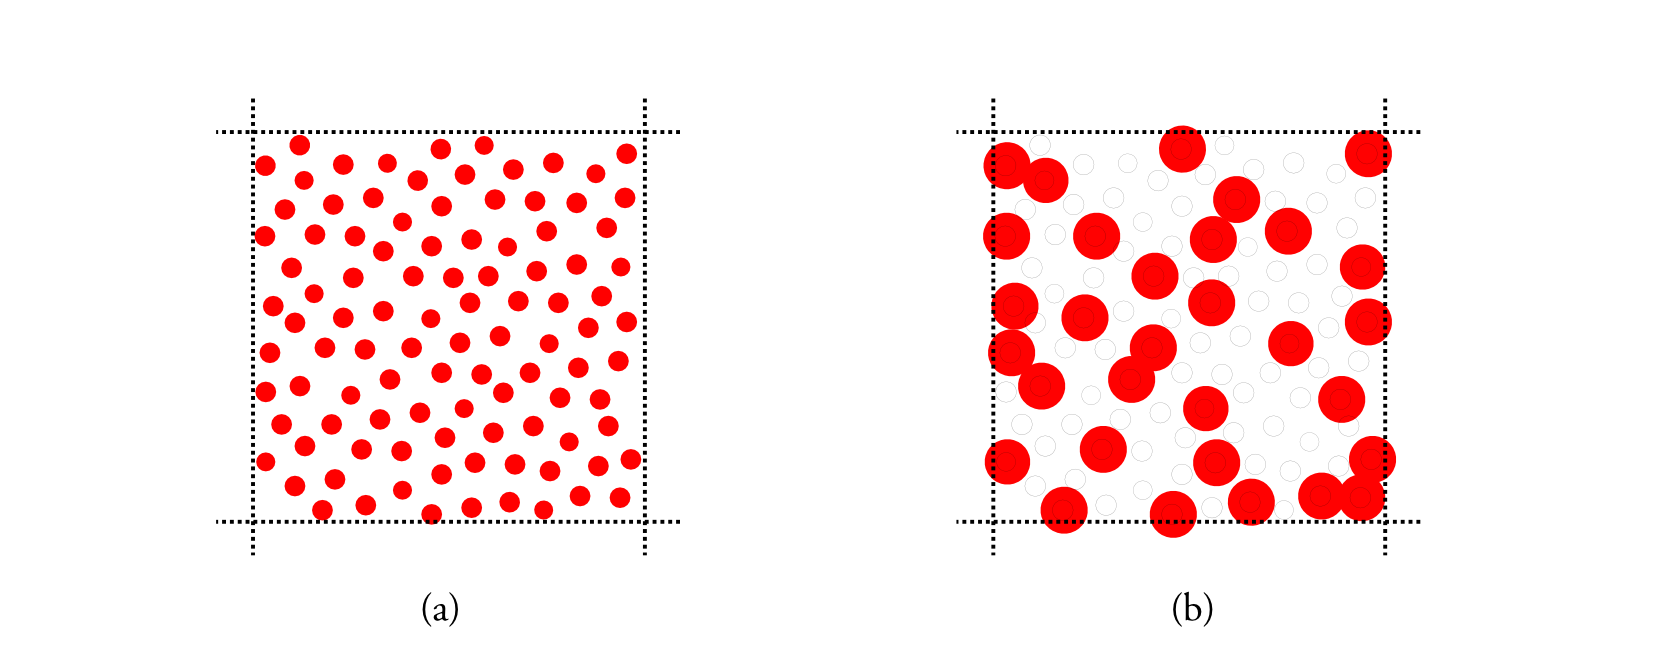
\includegraphics[width=\textwidth]{images/petites-primitives} 
					\caption{Primitives de taille négligeable}
					\label{fig:petit}
				\end{figure}
			Ceci est illustré au schéma (a) de la figure~\ref{fig:petit}, page~\pageref{fig:petit}, qui
			représente un pixel couvert de primitives d'aire inférieure à $\frac{1}{256}$ème de pixel.


			Plusieurs solutions ont été
			explorées :
			\begin{enumerate}
				\item[ignorer la primitive] Si celle-ci est isolée, cela ne posera pas de problème. Mais si
				de grandes surfaces, ou de longs traits sont composés de telles primitives, alors ceux-ci
				disparaitront à une certaine échelle. Le schéma (a) de la figure~\ref{fig:petit} illustre ce problème; chacune des primtives
				est trop petite pour modifier le pixel, mais prises ensembles, elles ont une contribution non
				négligable. L'algorithme de rasterisation évaluant les primitives une par une ne pourra se
				rendre compte de ce fait, et ce pixel sera rasterisé entièrement blanc.

				\item[colorer un minimum] Cette option consiste à faire contribuer toute primitive trop petite
				comme si elle avait une surface d'$\frac{1}{256}$eme de pixel, le minimum représentable. 

				Cela peut être une bonne solution pour les primitives isolées. Mais si le pixel est partiellement
				couvert par un grand nombre de ces primitives, le pixel sera trop fortement coloré. Cette solution
				mène inmanquablement à des artefacts innacceptables lors de la visualisation de l'image à grande échelle. 

				\item[une approche stochastique] Dans ce cas, soit la primitive contribue au pixel à un niveau
				d'intensité minimum $I_m$,  soit elle est ignorée, et ce avec une probabilité proportionelle à son aire. 
				
				Les grands ensembles de petites primitives sont ainsi représentés par des ensembles plus petits de 
				primitives de taille acceptable. 

				Ceci est représenté au schéma (b) de la figure~\ref{fig:petit}

				Il faut faire bien attention dans le choix du niveau minimum d'intensité $I_m$. Si ce niveau est
				choisi trop grand, le bruit de la sélection aléatoire deviendra visible. S'il est trop petit, 
				alors nous aurons un problème de quantisation des couelurs :

				Pronons l'exemple d'une primitive
				de couleur 
				\emph{(R,G,B) 8bit } $(255,120,60)$ et nous choisissons $I_m$ valant $\frac{1}{200}$ 
				
				La contribution en couleur de cette primitive sera donc de $(\frac{255}{200},\frac{120}{200},\frac{60}{200})$, soit
				quantisé sur 8bit $(1,0,0)$ La primitive orange apparaîtra donc rouge. 
				
				Il est malheureusement assez difficile de trouver un bon compromis entre bruit et qualité des couleurs. 
			\end{enumerate}

			Nous avons retenu comme solution d'ignorer les primitives, car cette méthode résout également le problème suivant
			pour lequel nous n'avons pas pu implémenter la solution.
			
			Enfin notons que ce problème devrait être nettement moins apparent lorsque l'on utilise des modèles 
			colorimétriques à 16 ou 32bit par canal.

		\subsubsection{Superposition des très petites primitves}
			L'approche qui consiste à remplir le pixel proportionellement à l'aire de la primitve ne fonctionne
			pas toujours lorsque l'on examine la contribution de plusieurs primitives à un seul pixel. 
			Si celles-ci ne se supperposent pas dans le pixel, alors les approches expliquées précédemment fonctionnent.
			Mais lorsque les opérations se supperposent, une erreur est commise.  Cette erreur est particulièrement
			flagrante lorsque l'écrat des brushes dans le trait est particulièrement petit puisque dans ce cas elles
			se superposent de manière importante.

				\begin{figure}[ht]
					\centering
					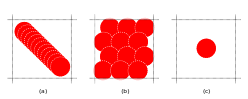
\includegraphics[width=\textwidth]{images/superposition-primitives} 
					\caption{Superposition de primitives dans un pixel}
					\label{fig:superposition}
				\end{figure}
			
			Ceci est illuststré à la figure~\ref{fig:superpositon}, page~\pageref{fig:superposition}. Les schémas (a) et (b)
			représentent chacun un pixel contenant le même nombre de primitives. Avec les approches précédentes, le trait (a)
			sera rasterisé avec l'intensité du cas (b).

			Une solution utilisée dans différents framework pour résoudre ce problème est de d'abord rasteriser le trait
			dans un buffer transparent intermédiaire dans lequel le mode de fusion utilisé pour la rasterisation des 
			brushes est le mode \emph{Maximum}. Au lieu de faire la somme des intensités, cet algorithme prend la maximum.  
			Le buffer intermédiaire est ensuite rasterisé avec le mode
			de fusion désiré sur le dessin.  Ainsi, la rasterisation d'un nombre quelquonque de primitives dans un seul pixel
			est considérée comme la rasterisation de la plus grande d'entre elles. 
			
			les situations des schémas (a) et (b) seront donc rasterisées comme (c). Dans le cas représenté sur le schéma, 
			l'erreur commise est de même intensité avec les deux méthodes. Cependant, comme vu précédemment il vaut mieux
			sous-estimer que sur-estimer les intensités. 

			Le mode de fusion \emph{Maximum} a d'autres avantages pour les primitives de plus grande taille: repasser 
			sur un trait n'augmente pas son intensité, ce qui facilite la peinture de large zones de manière uniforme. 

			Passer par un buffer intermédiaire peut se faire en utilisant une hlImage séparée pour chaque trait, il va
			donc de la responsabilité de l'utilisateur d'être au courant de cette solution et de l'utiliser lorsque cela
			est nécessaire. 
			
			Cette solution n'a pas été implémentée ou testée dans Himalaya car l'intégration entre le systême d'état et
			les opérations de fusion n'a pas été entièrement implémenté. 
			
			Si elle fonctionne dans les autres frameworks, il est en revanche difficile de savoir si elle fonctionnera 
			aussi bien dans des images utilisant à des différences d'échelle que ces frameworks ne peuvent atteindre. 
			
		\subsection{Problème de fusion à faible opacité}
			La fusion de primitives à faible opacité donne lieu à de fâcheux problèmes d'aliasing à cause de la quantisation.
			Le problème est exactement le même que les aberrations de couleurs pour les très petites primitives: Si l'on
			fait la fusion d'une primitve de couleur $(255,120,60)$ à 1\% d'opacité, on fera effectivement la fusion d'une
			primitive de couleur $(2,0,0)$. Ce qui est une très mauvaise approximation de la couleur désirée. 
			
			Ce problème apparait de manière d'autant plus flagrante lorsque de nombreuses primtives de faible opacité se
			superposent et que les erreurs s'accumulent. 

			La solution à ce problème utilisée par les autres frameworks consiste à passer par un buffer intermédiaire 
			dans lequel toutes les primitives du trait sont fusionnées à 100\% d'opacité. Ce buffer est ensuite fusionné
			sur le dessin à l'opacité désirée. 

			Cette solution n'a pas été testée ni implémentée pour les raisons expliquées précédamment.  

		\section{Oversampling}
			Une solution plus globale aux problème d'anti-aliasing est l'oversampling. Cette
			technique consite à effectuer la rasterisation avec une plus grande résolution dans les zones
			posant des difficultés d'anti-aliasing. 

			Le problème est donc l'identification des zones à oversampler. Une approche courante est l'utilisation
			d'un filtre de type gradient sur l'image finale afin de détecter les bords qui sont les principaux 
			endroits nécessitant l'oversampling. Malheureusement cette technique ne pourra pas identifier les zones
			où des détails trop petits ont simplement disparu.

			L'approche qui a été testée consiste à permettre à chaque opération de renvoyer un avis de qualité sur
			son résultat. Si cette qualité est insuffisante, l'on effectue le rendu
			du tile à résolution supérieure, c'est à dire les quatre tiles du niveau inférieur, que l'on met
			ensuite à l'échelle par interpolation linéaire. Ceci peut s'effectuer de manière récursive jusqu'à un degré
			maximum.

			Malheureusement cette technique implique une surcharge de travail dépassant les 400\%, ce qui ne permet plus
			des performances interactives. De plus, ceci ne permet d'augmenter la précision que d'un ou deux niveaux, ce
			qui n'est pas énorme pour des images gigapixel. 

			Cette solution peut cependant être considérée pour obtenir des rendus non interactifs de meilleure qualité.

		%\section{Problème de précision de positionement}

		%	Les paramètres de positionnement des primitives peuvent être décrits par des flottants ou des entiers. 
		%	Si l'on choisit les flottants, on peut avoir un positionnement avec une précision inférieure au pixel, ce qui
		%	est très pratique pour la réalisation de peintures.  L'inconvénient est qu'il est possible à une image gigapixel
		%	d'avoir une taille qui nécessite toute l'espace des entiers pour décrire les positions des pixels. Dans ce cas,
		%	les flottants n'ont plus la précision nécessaire pour pouvoir addresser chaque pixel indépendemment.  Le manque
		%	de précision peut atteindre plusieurs dixaines de pixels ce qui rend impossible la peinture. 

		%	Il n'y a pas de solution miracle à ce problème. Ainsi l'API peut proposer des primitives se positionant en 
		%	flottants et d'autres en entier. Cela laisse donc à l'utilisateur la responsabilité de choisir la méthode qui
		%	convient le mieux à son usage. 

\chapter{Test utilisateurs (10 pages) }
	\section{Procédure}
	\section{Résultats}
	\section{Analyse}
\chapter{Comparaison d'Himalaya aux autres frameworks}
\chapter{Conclusion}

